\documentclass[a4paper, 12pt, titlepage, fleqn]{article}

\usepackage[utf8]{inputenc}
\usepackage[T1]{fontenc}
\usepackage{times}
\usepackage{a4wide}
\usepackage{hyperref}
\usepackage{multirow}
%\usepackage{rail}
\usepackage{graphicx}
%\usepackage{amssymb}
%\usepackage{latexsym}
%\usepackage{amsmath}

%\railoptions{-t}

% bold emphasize in definitions
\newcommand{\dem}[1]{{\bf\em #1}}

% empty set confuses highlighting in vim
\newcommand{\set}[1]{\ensuremath{\left\{#1\right\}}}

\newcommand{\Ker}{\ensuremath{\operatorname{Ker}}}

\begin{document}

\title{
\includegraphics[scale=0.8]{images/logo.png} \vspace{5mm} \\ Advanced MAQL Reference\\version 1.0}
\author{}
\date{December 9, 2011}
\maketitle

\tableofcontents
\clearpage

\section*{Preface}
This reference contains a complete description of the Multi-Dimension Analytical Query Language (MAQL) used to manage projects and metrics in the GoodData platform. MAQL is a simple yet powerful query language that provides an underpinning of GoodData’s reporting capabilities. Its extension MAQL DDL (MAQL Data Definition Language) is used for building and adapting a data model. MAQL DQL (MAQL Data Query Language or metric language) is our flexible language for describing metrics in GoodData.

\section{Basic elements of GDC MAQL}

\subsection{Supported Data Types}
Below is a table giving you a rough idea on best practices. If you fall outside the boundaries, be sure to get in touch with us -- usually we can find a solution to work around problems. Specifically larger data sets (more rows) can be supported depending on how the data model is constructed and/or pre-aggregation can be used before data upload.\\

\begin{center}
\begin{tabular}{|l|l|} 
\hline
\textbf{\# of columns} & 60 attributes, references \& connection\_points \/ dataset \\ \hline
\textbf{Attribute size} & 128 characters by default, extensible to 256 characters\\ \hline
\multirow{4}{*}{\textbf{Fact size}} & \verb=DECIMAL(12,2)= by default ($-10^{10}..10^{10}$, \\ 
& 2 decimal places) \\ 
& extensible to \verb=DECIMAL(15,6)= by default ($-10^{9}..10^{9}$,\\ 
& 6 decimal places) \\ \hline
\end{tabular}\\
\end{center}

\subsection{Data Types used the GoodData Platform}
\label{datatypes}
By default the system automatically stores all facts as \verb=DECIMAL(12,2)= and all attributes and labels as 128-character strings. For performance reasons or to store other data types, you can redefine your column data type.\\

\begin{center}
\begin{tabular}{|l|l|l|} 
\hline
Data type & Description & Specific form \\ \hline
VARCHAR (\emph{n}) & \emph{n} $\epsilon$ $(1..255)$ & \\ 
DECIMAL (\emph{m},\emph{d}) & \emph{m}: \emph{min}($-10^{15}$), \emph{max}($10^{15}$), \emph{d}: max = 6 & \\
INT & \emph{min}($-2147483648$),\emph{max}($2147483647$) & \\
BIGINT & \emph{min}($-10^{15}$), \emph{max}($10^{15}$) & \\
DATE &  & 'YYYY-MM-DD'	 \\
DOUBLE & discouraged & \\ \hline
\end{tabular}\\

\end{center}

The DATE datatype automatically maps with the GoodData-provided date dimension, if you have previously included it into the project.

\subsection{GDC Objects}
\subsubsection{Identifiers}
Identifiers in MAQL are denoted by {curly brackets}. Once an object is created, the identifier is persistent and cannot be changed. You can choose your own naming conventions for identifiers (in the examples below we often put identifiers into "namespace" by prefixing them with "folder.", "fact." etc.) Identifiers can contain alphanumeric characters, underscore and dot (e.\,g. [A-Za-z0-9\_\textbackslash .]).

\subsubsection{LDM Objects}

LDM (Logical Data Model) describes the logical structure an organization's data in terms like datasets, attributes and facts. While the LDM is representing the logical structure, the physical structure is defined as PDM (Physical Data Model). 

The LDM is necessary for creating your reports. It consists of attributes and facts that GoodData users add to their reports. Besides attributes and facts, LDM includes also datasets and folders. Simple example is shown on the schema bellow. 

\begin{figure}[htb]
\centering
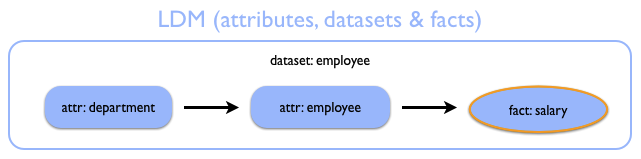
\includegraphics[scale=0.5]{images/ldm-model.png}
\caption{Example of simple LDM}
\label{fig:ldm}
\end{figure}

As you can see, the LDM contains one fact and two attributes in a hierarchy (department and employee). As we have mentioned above, we'll use the MAQL DDL language to define the LDM.

\paragraph*{Attributes} An attribute is the unit that allows you to specify how to aggregate (or slice) your data. Examples would include: Assignee, City, Day, ID, Group etc. Attributes can optionally have additional labels. These are alternate string representation of the same semantic value. For example a person John Doe is the same person, regardless if they are visualized as "J. Doe", "Doe, John", "Johnny" etc. Or "Jan 10", "January 2010" and "01/2010".

\paragraph*{Attribute IDs} Every attribute has its own unique number. The number is invisible to end users. However, you can rely on the creation rules in regards to attribute IDs. In the specific case of date values, the ordinal attribute IDs are ordered by the attribute value. So, the Month attribute value of May 2007 is higher than the ID value of April 2007. Therefore, the relational operators (>,<,>=,<=,=) can be applied to the attribute IDs. So the filter \verb=WHERE Month > April 2007= returns all months after April 2007.

\paragraph*{Facts} A fact is a data column containing computational data - e.\,g. prices, amounts. Generally, facts are measurable items of data attached to each record in the source data. Facts are always numbers, and cannot be broken down further. Examples include: Sales (a price for one transaction), Salary (the amount of money received), Cost (the amount paid for an item, Items Shipped (the number of items shipped in one delivery), etc. These are amounts reflected in each “transaction” or record.

\paragraph*{Datasets} A dataset is one joint source of data and comprises of attributes and facts.

\paragraph*{Folders} Top-level categories for organizing attributes or hierarchies of attributes. For example, you can create a Time folder containing the Year, Quarter, Month and Day attributes. 
Folders are used to visually organize facts or attributes and metrics for the user. Folders are types - e.\,g. they can only contain objects of one kind (hence the TYPE section). Folders are used to organize attributes and facts visually for users.

\subsubsection{PDM Mapping}

The PDM is used for the data storage and query. It is de-facto a DBMS schema (tables, columns, primary/foreign keys etc.). 

Most analytical tools and platforms will force you to develop both LDM and PDM that are perfectly aligned. Unlike the average tools, the GoodData interface with user only via the LDM. The corresponding PDM is automatically generated from the LDM. The LDM model is created and modified via the MAQL DDL language statements, that are described in the section \ref{DDL} of this reference.

The figure below outlines the PDM that has been automatically generated from the LDM above LDM (Fig.~\ref{fig:ldm}).

\begin{figure}[htb]
\centering
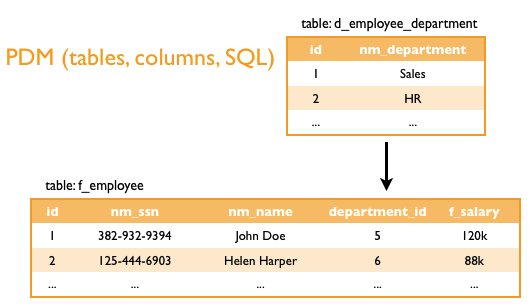
\includegraphics[scale=0.6]{images/pdm-model.png}
\caption{Generated PDM from LDM}
\label{fig:pdm}
\end{figure}

As we mentioned before, the PDM is standard DBMS schema with tables, columns, primary and foreign keys. A LDM \verb=ATTRIBUTE= is represented by a database table with primary key and couple text columns (one for each \verb=LABEL=) in the PDM. A LDM \verb=FACT= is mapped to a column in a PDM fact table. The figure below outlines the PDM that has been automatically generated from the LDM above.

Once we have the LDM, the PDM and DLI (Data Loading Interface) will be generated automatically via the SYNCHRONIZE MAQL DDL command. 
The DLI is used for loading data to the PDM.

The GoodData platform loads data in self-describing packages. The data package is a ZIP archive that contains the data (delimited file) and a manifest that describes how the data map to the project's LDM and PDM. The figure below shows the data file only. As you can see this is de-normalized (flattened \verb=d_employee_department= and \verb=f_employee= PDM tables) version of the PDM.

\begin{figure}[htb]
\centering
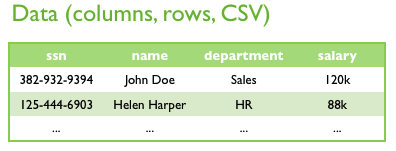
\includegraphics[scale=0.6]{images/data-template.png}
\caption{De-normalized version of PDM}
\label{fig:pdm}
\end{figure}

\section{Operators}
\label{operators}
Logical and special operators
\paragraph*{= (equals)} This filter allows you to compute the metric from a specific attribute value.

\textbf{\emph{syntax}}  \hspace{.9cm}\verb=SELECT project_metric= 

\hspace{2.2cm}\verb=WHERE {project_attribute}= = \verb={project_attribute_value}=

\textbf{\emph{example}}  \hspace{.9cm}\verb=SELECT Salary WHERE Year= = \verb=2007;=

\textbf{\emph{example}}  \hspace{.9cm}\verb=SELECT Revenues WHERE Month= = \verb={This};=

\textbf{\emph{example}}  \hspace{.9cm}\verb=SELECT Expenses WHERE Quarter= = \verb={Previous};=

\textbf{\emph{example}}  \hspace{.9cm}\verb=SELECT Expenses WHERE Quarter= = \verb={This} - 2;=

\textbf{\emph{example}}  \hspace{.9cm}\verb=SELECT Amount WHERE Date ordered= = \verb=Date Shipped;=

\textbf{\emph{example}}  \hspace{.9cm}\verb=SELECT Employee WHERE Payment= = \verb=10000;=

\paragraph*{<> (does not equal)} This filter allows you to compute the metric by excluding a particular attribute value.

\textbf{\emph{syntax}}  \hspace{.9cm}\verb=SELECT project_metric;=

\hspace{2.2cm}\verb=WHERE {project_attribute} <> {project_attribute_value};=

\textbf{\emph{example}}  \hspace{.9cm}\verb=SELECT Revenues WHERE Year <> 2006;=

\textbf{\emph{example}}  \hspace{.9cm}\verb=SELECT Amount WHERE Date Ordered <> Date Shipped;=

\paragraph*{IN}
This filter allows you to compute the metric from multiple attribute values.

\textbf{\emph{syntax}}  \hspace{.9cm}\verb=SELECT project_metric=

\hspace{2.2cm}\verb=WHERE {project_attribute}=

\hspace{2.2cm}\verb=<> (proj_attr_val1, proj_attr_val2);=

\textbf{\emph{example}}  \hspace{.9cm}\verb=SELECT Profit WHERE Year IN (2006, 2007);=


\paragraph*{NOT IN}
This filter allows you to compute the metric by excluding particular attribute values.

\textbf{\emph{syntax}}  \hspace{.9cm}\verb=SELECT project_metric=

\hspace{2.2cm}\verb=WHERE {project_attribute}=

\hspace{2.2cm}\verb=NOT IN (project_attribute_value1, project_attribute_value2);=

\textbf{\emph{example}}  \hspace{.9cm}\verb=SELECT Profit WHERE Year NOT IN (2006, 2007);=

\textbf{\emph{example}}  \hspace{.9cm}\verb=SELECT Sales WHERE Quarter NOT IN ({This}, {Previous});=

\paragraph*{BETWEEN} This filter allows you to compute the metric by using attribute values from a specified range (including endpoints).

\textbf{\emph{syntax}}  \hspace{.9cm}\verb=SELECT project_metric=

\hspace{2.2cm}\verb=WHERE {project_attribute}=

\hspace{2.2cm}\verb=BETWEEN project_attribute_value1 =

\hspace{2.2cm}\verb=AND project_sttribute_value2;=

\textbf{\emph{example}}  \hspace{.9cm}\verb=SELECT Profit WHERE Year BETWEEN 2005 AND 2008;=

\textbf{\emph{example}}  \hspace{.9cm}\verb=SELECT Sales WHERE Quarter BETWEEN {This} - 5 AND {This});=


\paragraph*{NOT BETWEEN} This filter allows you to compute the metric by using attribute values outside of a specified range (excluding endpoints).

\textbf{\emph{syntax}}  \hspace{.9cm}\verb=SELECT project_metric=

\hspace{2.2cm}\verb=WHERE {project_attribute}=

\hspace{2.2cm}\verb=NOT BETWEEN project_attribute_value1 =

\hspace{2.2cm}\verb=AND project_sttribute_value2;=

\textbf{\emph{example}}  \hspace{.9cm}\verb=SELECT Profit WHERE Year NOT BETWEEN 2005 AND 2008;=

You can use these clauses to create fixed numbers which can be used in other computations to create complex metrics. Fixing numbers is achieved by locking the aggregation level to an attribute in one or more dimensions.

\section{Functions and macros}

All the available functions and macros are handling time comparisons and global operations with time dimensions.

\subsection{Functions FOR Previous, FOR PreviousPeriod}
\label{functions}
Two special functions in MAQL allow you to create metrics showing a time over time comparison (e.\,g., month over month, or quarter over quarter): 

\hspace{0.9cm}\verb=FOR Previous()= and 

\hspace{0.9cm}\verb=FOR PreviousPeriod()=.

\paragraph*{FOR Previous ()} This statement allows you to compute a metric for a previous, fixed time period.

\textbf{\emph{example}}  \hspace{.9cm}\verb=SELECT Revenues FOR Previous(Quarter);=

\noindent This example result is shown on the figure below. As you can see it provides the value from previous period, in this example is the previous quarter.

\begin{figure}[htb]
\centering
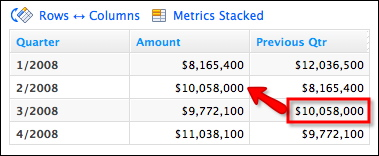
\includegraphics[scale=0.6]{images/rg_prevQtr.png}
\caption{SELECT Revenues FOR Previous(Quarter)}
\label{fig:4pq}
\end{figure}

\textbf{\emph{example}}  \hspace{.9cm}\verb=SELECT Revenues FOR Previous(Quarter,1);=

\noindent This example result is shown on the figure \ref{fig:4pq2}. In this second example, the extra "1" specifies to skip back two quarters, rather than simply last quarter.

\begin{figure}[htb]
\centering
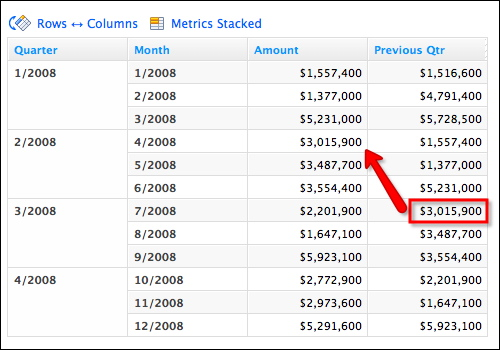
\includegraphics[scale=0.6]{images/rg_prevQtrMonth.png}
\caption{SELECT Revenues FOR Previous(Quarter,1)}
\label{fig:4pq2}
\end{figure}

\paragraph*{FOR PreviousPeriod()} This statement allows you to compute a metric for a contextual previous period.

\textbf{\emph{example}}  \hspace{.9cm}\verb=SELECT Payment FOR PreviousPeriod(Quarter);=

\noindent Both of the example's results are shown on the figure below. As you can see it provides the value from previous period, in this example is the previous quarter. In this second example, the extra "1" specifies to skip back two periods, rather than simply the previous period.

\textbf{\emph{example}}  \hspace{.9cm}\verb=SELECT Payment FOR PreviousPeriod(Quarter,1);=\\

\begin{figure}[htb]
\centering
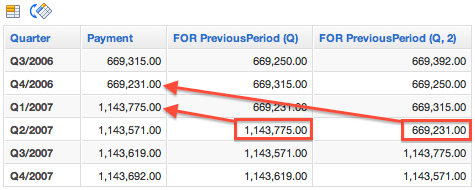
\includegraphics[scale=0.6]{images/4pp2.png}
\caption{Payment FOR Previous(Quarter) and FOR Previous(Quarter,2)}
\label{fig:4pq2}
\end{figure}

\paragraph*{The Difference Between FOR Previous() and FOR PreviousPeriod()\\}

The \verb=FOR Previous()= statement will always return the previous aggregated result for the time period specified within the parenthesis. For example, entering \verb=FOR Previous(Year)= will always return the metric aggregated for the previous year, based on the values in the report. For example, with current sales of April 2010, FOR Previous(Year) will display April 2009. Likewise, FOR Previous(Quarter) will display January 2010 (e.\,g., since April is M1/Q2, the "Previous()" function would look for M1/Q1 -- the previous quarter -- or January 2010).

\begin{figure}[htb]
\centering
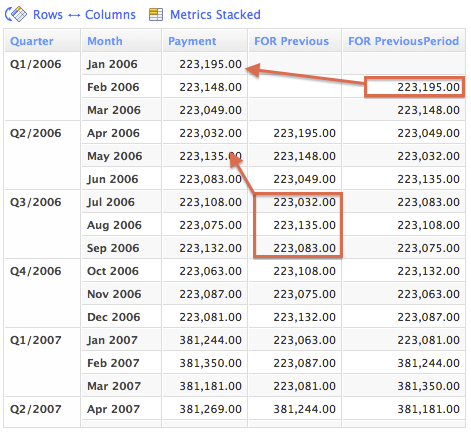
\includegraphics[scale=0.6]{images/4pr4pp.png}
\caption{The difference between FOR Previous() and FOR PreviousPeriod()}
\label{fig:4pp}
\end{figure}

On the other hand, \verb=FOR PreviousPeriod()= will adjust the aggregation level of the returned metric based on the attributes contained within the report. For example, if Quarter is displayed in the report, the Previous Period would also be preceding Quarter. If this changes to Year, then the Previous Period would also change to the preceding Year. However, it is still necessary to specify an attribute within parenthesis so that the metric knows from which date dimension to select the previous period.

\subsubsection{FOR Next() and FOR NextPeriod()}
Alternatively, it is also possible to compare against future dates using two other special MAQL functions:

\hspace{0.9cm}\verb=FOR Next()= and 

\hspace{0.9cm}\verb=FOR NextPeriod()=. 

Both of these constructs function in the same was as \verb=FOR Previous()=\\ and \verb=FOR PreviousPeriod()= above.

\paragraph*{FOR Next()}
This statement allows you to compute a metric for a future, fixed time period.

\textbf{\emph{example}}  \hspace{.9cm}\verb=SELECT Revenues FOR Next(Quarter);=

Again as in \verb=FOR Previous()= function, if we add "2" as second function parameter, it specifies to jump ahead two quarters, rather than simply next quarter.

\textbf{\emph{example}}  \hspace{.9cm}\verb=SELECT Revenues FOR Next(Quarter,2);=

\paragraph*{FOR NextPeriod()}
This statement allows you to compute a metric for a contextual next period.

\textbf{\emph{example}}  \hspace{.9cm}\verb=SELECT Revenues FOR NextPeriod(Quarter);=

Again, as in FOR PreviousPeriod() function, if we add "2" as second function parameter, it specifies to jump ahead two quarters, rather than simply next quarter.

\textbf{\emph{example}}  \hspace{.9cm}\verb=SELECT Revenues FOR NextPeriod(Quarter,2);=

\subsection{Time macros {This}, {Previous}} 
\label{timemcr}
MAQL provides special constructs for specifying days in your reports. We define them as time macros and allow you to use create reports for "Today" or "Yesterday", and can also help create Year-to-Date reports.

The time macros can be used as attribute values for attributes contained in the GoodData Date hierarchy. These commands take inherit their value based on their context within the metric.

\begin{itemize}
\item In this example, \{This\} would mean "This Date," or "Today".

\textbf{\emph{example}}  \hspace{.9cm}\verb=SELECT Payment WHERE Date= = \verb={This};=

\item In this example, \{This\} - 1 would mean "This Date" minus one, or "Yesterday".

\textbf{\emph{example}}  \hspace{.9cm}\verb=Example: SELECT Payment WHERE Date= = \verb={This} - 1;=

\item In this example, \{This\} would mean "This Month".

\textbf{\emph{example}}  \hspace{.9cm}\verb=SELECT Payment WHERE Month= = \verb={This};=

\item In this example, \{Previous\} would mean "Previous Quarter".

\textbf{\emph{example}}  \hspace{.9cm}\verb=SELECT Expenses WHERE Quarter= = \verb={Previous};=

\item In this example, \{This\} would mean "This Year".

\textbf{\emph{example}}  \hspace{.9cm}\verb=SELECT Payment WHERE Year= = \verb={This};=

\item In this example, the first \{This\} would mean "This Year" while the second \{This\} would refer to "This Day of Year" (e.\,g., Day 1 for Jan. 1, Day 2 for Jan. 2, etc).

\textbf{\emph{example}}  \hspace{.9cm}\verb=SELECT Payment WHERE Year= = \verb={This}=

\hspace{2.5cm}\verb=AND Day of Year= = \verb={This};=

\item In this example, \{Previous\} would mean "Previous (Last) Quarter" and \{This\} would refer to "Today as a numeric Day of the Quarter" (e.\,g., Day 62 of the quarter).

\textbf{\emph{example}}  \hspace{.9cm}\verb=SELECT # of Employees WHERE Quarter= = \verb={Previous}=

\hspace{2.5cm}\verb=AND Day of Quarter= = \verb={This};=
\end{itemize}

\section{Expressions}
\subsection{Logical expressions}
\label{logical}
Allow you to combine multiple filters.

\paragraph*{NOT} If you specify a filter and precede it with NOT, then everything that is specified by the filter will be excluded from the report computation.

\textbf{\emph{example}}  \hspace{.9cm}\verb=SELECT Revenues WHERE NOT (Year= = \verb=2006 AND Month= = \verb=5);=

\paragraph*{AND} If you combine filters using AND, then both filters are applied when computing the metric.

\textbf{\emph{example}}  \hspace{.9cm}\verb=SELECT Revenues WHERE Year= = \verb=2006 AND Month= = \verb=5;=

\paragraph*{OR} If you combine filters using OR, then the result for each filter is computed individually and the results are combined.

\textbf{\emph{example}}  \hspace{.9cm}\verb=SELECT Revenues WHERE Year= = \verb=2006 OR Year= = \verb=2005;=

\section{Common MAQL DDL Clauses}
\label{DDL}

All the DDL statements are used when you creating your project with the CL tool. But you can use them also on the project's gray pages. The command line for running the DDL statements is located on the following URL

\verb=https://secure.gooddata.com/gdc/md/<project_id>/ldm/manage=

\subsection{Create statement}

The MAQL DDL is used to create the LDM. Such LDM is shown on the Fig.~\ref{fig:hrldm}. This model was simplified for better understanding, only some of the date related attributes are displayed.

\begin{figure}[htb]
\centering
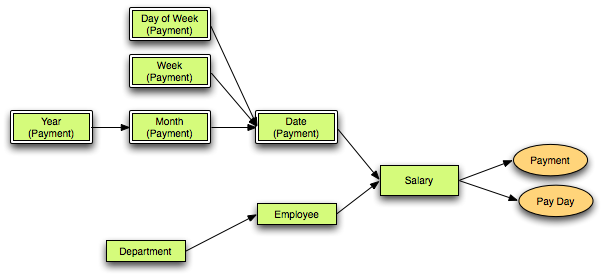
\includegraphics[scale=0.6]{images/hr_simple.png}
\caption{HR demo project LDM}
\label{fig:hrldm}
\end{figure}

\subsubsection{Create attributes}
An attribute is represented by a database table with a primary key and couple text columns. Attributes are categories that are used for slicing and dicing the facts (countable numbers). An attribute can be empty or with keys and labels. Creating attributes with primary and foreign keys allows us to construct the LDM as on Fig.~\ref{fig:hrldm}. If we create attribute Employee with this statement:

\textbf{\emph{example}}  \hspace{.9cm}\verb=CREATE ATTRIBUTE {attr.employee.employee}=

\hspace{2.5cm}\verb=VISUAL(TITLE "Employee", FOLDER {dim.employee}) =

\hspace{2.5cm}\verb=AS KEYS {f_employee.id} FULLSET;=\\

\noindent This statement creates the LDM attribute named \verb=Employee=. The LDM attribute maps to a PDM table that has the primary key \verb={f_employee.id} (FULLSET)=. The key word FULLSET marks the LDM attribute which is defined in the PDM as primary key. We can also add the foreign key, but we will show it later. The attribute is defined as a PDM table. The attribute itself is the auto-generated ID \verb=f_employee.id=. 

Now, we will create the Department attribute and we'll create the foreign key to the \verb=f_employee= table:

\textbf{\emph{example}}  \hspace{.9cm}\verb=CREATE ATTRIBUTE {attr.employee.department}=

\hspace{2.5cm}\verb=VISUAL(TITLE "Department")= 

\hspace{2.5cm}\verb=AS KEYS {d_employee_department.id} FULLSET,=

\hspace{2.5cm}\verb={f_employee.department_id};=

\noindent Note that the MAQL DDL statement contains two keys. The first one \verb=d_employee_department.id= is the primary key and the second one \verb=f_employee.department_id= is the foreign key that ties the \verb=d_employee_department= table to the \verb=f_employee= table.

\paragraph*{Create attribute full syntax} The full syntax of the attribute creation command is specified as

\textbf{\emph{syntax}}  \hspace{.9cm}\verb=CREATE ATTRIBUTE {identifier}=

\hspace{2.2cm}\verb=[VISUAL({properties}) [HYPERLINK]=

\hspace{2.2cm}\verb=AS {identifier} KEYS {object} KEY_TYPE]=

\hspace{2.2cm}\verb=WITH LABELS {label_list} ORDER {identifier}=

\hspace{2.2cm}\verb=[ASC | DESC];=

\noindent Create empty attribute.

\textbf{\emph{example}}  \hspace{.9cm}\verb=CREATE ATTRIBUTE {attr.employee.name}=

\hspace{2.5cm}\verb=VISUAL(TITLE "Name",=

\hspace{2.5cm}\verb=FOLDER {folder.employee}) AS;=

\noindent Create attribute with primary key.

\textbf{\emph{example}}  \hspace{.9cm}\verb=CREATE ATTRIBUTE {attr.employee.employee}=

\hspace{2.5cm}\verb=AS {f_employee.id} FULLSET;=

\noindent Create attribute with label.

\textbf{\emph{example}}  \hspace{.9cm}\verb=CREATE ATTRIBUTE {attr.employee.name}=

\hspace{2.5cm}\verb=AS WITH LABELS {label.employee.name}=

\hspace{2.5cm}\verb=VISUAL(TITLE "Employee's name");=

\noindent For the rest of the example in this section we will work with opportunities. First, we create attribute with title and mapping for primary key and with label \emph{Opp. category} mapped to column in the same table.

\textbf{\emph{example}}  \hspace{.9cm}\verb=CREATE ATTRIBUTE {attr.opportunity.category}=

\hspace{2.5cm}\verb=VISUAL(TITLE "Category of opportunity",=

\hspace{2.5cm}\verb=FOLDER {folder.opportunity}) =

\hspace{2.5cm}\verb=AS KEYS {tab_cat.col_id} FULLSET, {tab_opp.col_cat}=

\hspace{2.5cm}\verb=WITH LABELS {label.opportunity.category}=

\hspace{2.5cm}\verb=VISUAL(TITLE "Opp. category") AS {tab_cat.col_lbl};=

\noindent Create attribute with order (sorting options on attributes).

\textbf{\emph{example}}  \hspace{.9cm}\verb=CREATE ATTRIBUTE {attr.opportunity.category}=

\hspace{2.5cm}\verb=AS LABELS {label1} VISUAL(TITLE "Opp. category")=

\hspace{2.5cm}\verb=ORDER {label1} ASC;=

\textbf{\emph{example}}  \hspace{.9cm}\verb=CREATE ATTRIBUTE {attr.employee.employee}=

\hspace{2.5cm}\verb={attr.employee.firstname} VISUAL(TITLE “First Name”)=

\hspace{2.5cm}\verb=ORDER {attr.employee.firstname} DESC;=

\noindent To allow attribute to be shown as hyperlink.

\textbf{\emph{example}}  \hspace{.9cm}\verb=CREATE ATTRIBUTE {attr.employee.web}=

\hspace{2.5cm}\verb=AS LABELS {attr.employee.web}=

\hspace{2.5cm}\verb=VISUAL(TITLE “First Name”) HYPERLINK;=

If we’ll create the foreign key to the \verb=f_employee= table, note that the first MAQL DDL statement contains two keys. The first one \verb=d_employee_department.id= is the primary key and the second one \verb=f_employee.department_id= is the foreign key that ties the\\ \verb=d_employee_department= table to the \verb=f_employee= table.

\textbf{\emph{example}}  \hspace{.9cm}\verb=CREATE ATTRIBUTE {attr.employee.department}=

\hspace{2.5cm}\verb=VISUAL(TITLE "Department")=

\hspace{2.5cm}\verb=AS KEYS {d_employee_department.id}=

\hspace{2.5cm}\verb=FULLSET, {f_employee.department_id};=

\subsubsection{Create dataset}
Dataset groups all following logical model elements together.

\textbf{\emph{syntax}}  \hspace{.9cm}\verb=CREATE DATASET {identifier}=

\hspace{2.1cm}\verb=[VISUAL({properties})];=

\noindent To create empty dataset. Create dataset with label \emph{Employee} .

\textbf{\emph{example}}  \hspace{.9cm}\verb=CREATE DATASET {dataset.employee}=

\hspace{2.5cm}\verb=VISUAL(TITLE "Employee");=

\subsubsection{Create facts}
Its purpose is to create fact with or without expression. Again, if we use our LDM from fig.~\ref{fig:hrldm}, we can add to our  employees salary fact:

\textbf{\emph{example}}  \hspace{.9cm}\verb=CREATE FACT {fact.employee.salary}=

\hspace{2.5cm}\verb=VISUAL(TITLE "Salary")=

\hspace{2.5cm}\verb=AS {f_employee.f_salary};=

This statement creates new Salary fact (LDM) and the corresponding \verb={f_salary}= column in the \verb=f_employee= table (PDM). Remember that the fact is represented as a database column.

After successful creation, the fact must be added to the employee dataset:

\textbf{\emph{example}}  \hspace{.9cm}\verb=ALTER DATASET {dataset.employee}=

\hspace{2.5cm}\verb=ADD {fact.employee.salary};=

All PDM tables, columns, keys etc. are automatically generated after calling the \verb=SYNCHRONIZE= MAQL DDL command that is usually the last command of a MAQL DDL script.

\textbf{\emph{syntax}}  \hspace{.9cm}\verb=CREATE FACT {identifier}=

\hspace{2.1cm}\verb=[VISUAL({properties})];=

\hspace{2.1cm}\verb=AS [{object}];=

\noindent Create empty fact.

\textbf{\emph{example}}  \hspace{.9cm}\verb=CREATE FACT {fact.opportunity.sales}=

\hspace{2.5cm}\verb=VISUAL( TITLE "Sales" ) AS;=

\noindent Create fact with expression.

\textbf{\emph{example}}  \hspace{.9cm}\verb=CREATE FACT {fact.opportunity.sales}=

\hspace{2.5cm}\verb=VISUAL( TITLE "Sales" ) AS {tab_opp.col_sales};=

\subsubsection{Create folder}
Create the folders that group attributes and facts. Folders keep our dataset readable and organized.

\textbf{\emph{syntax}}  \hspace{.9cm}\verb=CREATE FOLDER {identifier}=

\hspace{2.1cm}\verb=[VISUAL({properties})]=

\hspace{2.1cm}\verb=TYPE {type_identificator};=

\noindent Create folder of attributes.

\textbf{\emph{syntax}}  \hspace{.9cm}\verb=CREATE FOLDER {dim.employee}=

\hspace{2.2cm}\verb=VISUAL(TITLE "Employee Title") TYPE ATTRIBUTE;=

\noindent Create folder of facts.

\textbf{\emph{example}}  \hspace{.9cm}\verb=CREATE FOLDER {ffld.salary}=

\hspace{2.5cm}\verb=VISUAL(TITLE "Salary") TYPE FACT;=

\noindent  Create folder of metrics.

\textbf{\emph{example}}  \hspace{.9cm}\verb=CREATE FOLDER {ffld.salary}=

\hspace{2.5cm}\verb=VISUAL(TITLE "Salary", DESCRIPTION "salary description")=

\hspace{2.5cm}\verb=TYPE METRIC;=

\subsubsection{Create metric}
Not supported in MAQL DDL. The recommended way to create metrics is inside the GoodData platform by using metric editor (see section \ref{metrics})

\subsection{Alter statement}
The ALTER statements allows you to make changes in the LDM model.

\subsubsection{Alter attribute}
\label{alter}
To change attribute property as visual as key or label. The attribute has to exists.

\textbf{\emph{syntax}}  \hspace{.9cm}\verb=ALTER ATTRIBUTE {identifier}=

\hspace{2.2cm}\verb=[VISUAL({properties})]=

\hspace{2.2cm}\verb=[[DEFAULT LABEL {identifier}] | [ DROP [KEYS |=

\hspace{2.2cm}\verb=LABELS] [ADD [KEYS [PRIMARY | FULLSET] |=

\hspace{2.2cm}\verb=LABELS] | ALTER LABEL {identifier} [HYPERLINK]]=

\hspace{2.2cm}\verb= {object} ORDER BY {identifier} [ DESC | ASC ];=

\noindent Add three keys to attribute (first is primary).

\textbf{\emph{example}}  \hspace{.9cm}\verb=ALTER ATTRIBUTE {dataset.salary}=

\hspace{2.5cm}\verb=ADD KEYS {dt.salary.payday_id} PRIMARY,=

\hspace{2.5cm}\verb={dt.salary.payday}, {dt.salary.employee};=

\noindent Add label with identifier \emph{label.employee.employee} and definition \emph{attr.employee.employee}.

\textbf{\emph{example}}  \hspace{.9cm}\verb=ALTER ATTRIBUTE {attr.employee.employee}=

\hspace{2.5cm}\verb=ADD LABELS {label.employee.employee}=

\hspace{2.5cm}\verb=AS {f_employee.nm_employee};=

\noindent Drop key which identify the employee name from employee's attribute.

\textbf{\emph{example}}  \hspace{.9cm}\verb=ALTER ATTRIBUTE {attr.employee.employee}=

\hspace{2.5cm}\verb=DROP KEYS {d_employee.id};=

\noindent Drop all keys from attribute.

\textbf{\emph{example}}  \hspace{.9cm}\verb=ALTER ATTRIBUTE {attr.employee.employee}=

\hspace{2.5cm}\verb=DROP KEYS ALL;=

\noindent To change attribute title and folder.

\textbf{\emph{example}}  \hspace{.9cm}\verb=ALTER ATTRIBUTE {attr.employee.employee}=

\hspace{2.5cm}\verb=VISUAL(FOLDER {dim.employee}, TITLE "Employee");=

\noindent To change title of two attribute's labels.

\textbf{\emph{example}}  \hspace{.9cm}\verb=ALTER ATTRIBUTE {attr.company}=

\hspace{2.5cm}\verb=ALTER LABELS {label.company.company.fullname}=

\hspace{2.5cm}\verb=VISUAL(TITLE "GoodData Corporation"),=

\hspace{2.5cm}\verb={label.company.company.shortname} VISUAL(TITLE "GDC");=

\noindent To change ORDER.

\textbf{\emph{example}}  \hspace{.9cm}\verb=ALTER ATTRIBUTE {attr.employee.employee}=

\hspace{2.5cm}\verb=ORDER BY {label.employee.employee.firtsname} ASC;=

\noindent To change DEFAULT.

\textbf{\emph{example}}  \hspace{.9cm}\verb=ALTER ATTRIBUTE {attr.employee.employee}=

\hspace{2.5cm}\verb=DEFAULT LABEL {label.employee.employee};=

\noindent To allow attribute to be shown as a hyperlink.

\textbf{\emph{example}}  \hspace{.9cm}\verb=ALTER ATTRIBUTE {attr.employee.web}=

\hspace{2.5cm}\verb=DEFAULT ALTER LABELS {attr.employee.web} HYPERLINK;=

\subsubsection{Alter dataset}
To add or drop objects (attributes, facts) to/from dataset. Or only change visual property of dataset. One attribute or fact should always belong to exactly one dataset (no more, no less). Otherwise the validation of the project will fail.

\textbf{\emph{syntax}}  \hspace{.9cm}\verb=ALTER DATASET {identifier}=

\hspace{2.2cm}\verb=[VISUAL({properties})]=

\hspace{2.2cm}\verb=[OPERATION {objects}];=

\noindent Add fact or attribute to dataset.

\textbf{\emph{example}}  \hspace{.9cm}\verb=ALTER DATASET {dataset.quotes}=

\hspace{2.5cm}\verb=ADD {probability};=

\noindent Add a new attribute into the dataset.

\textbf{\emph{example}}  \hspace{.9cm}\verb=ALTER DATASET {dataset.employee}=

\hspace{2.5cm}\verb=ADD {attr.employee.employee};=

If we'll create the foreign key to the \verb=f_employee table=, note that the first MAQL DDL statement contains two keys. The first one \verb=d_employee_department.id= is the primary key and the second one \verb=f_employee.department_id= is the foreign key that ties the \verb=d_employee_department= table to the \verb=f_employee= table.\\

\noindent Drop attribute from dataset.

\textbf{\emph{example}}  \hspace{.9cm}\verb=ALTER DATASET {dataset.quotes}=

\hspace{2.5cm}\verb=DROP {Cutomer};=

\noindent Change title of dataset.

\textbf{\emph{example}}  \hspace{.9cm}\verb=ALTER DATASET {dataset.quotes}=

\hspace{2.5cm}\verb=VISUAL(TITLE "Internal Quotes Data");=

\subsubsection{Alter datatype}
This statement allows change data type of DataLoadingColumn (DLC). DLC is a column that is exposed to user API and represents column in user's CSV file. Data column identifiers is the only exception, where identifier name has to follow a certain structure. These identifiers reference specific data columns in the data files that you upload through the upload API. The identifiers must take form of \verb=file.column=. The \verb=file= part corresponds to the data file, while column corresponds to a specific column. All columns that in 3NF share a common file must also share the same prefix in their identifiers. A LDM is defined through MAQL statements, where the \verb=table.column= is specified for the mapping on PDM. Within that MAQL statement the \verb=table.column= identifier is handled as DataLoadingColumn (DLC) and concurrently PDM objects table and column are established. 

By default the system automatically stores all facts as \verb=DECIMAL(12,2)= and all attributes and labels as 128-character strings. For performance reasons or to store other data types, you can redefine your column data type (supported data types see section \ref{datatypes}).

\textbf{\emph{syntax}}  \hspace{.9cm}\verb=ALTER DATATYPE {object.identifier}=

\hspace{2.2cm}\verb={supported_datatype};=

\noindent Changing data type at three columns of the employee table.

\textbf{\emph{example}}  \hspace{.9cm}\verb=ALTER DATATYPE {dataset.employee.empl_id} INT,=

\hspace{2.5cm}\verb={dataset.employee.empl_name} CHAR(100),=

\hspace{2.5cm}\verb={dataset.employee.empl_fact} DECIMAL(10,2);=

\subsubsection{Alter fact}
When we need to change visual or expression property.

\textbf{\emph{syntax}}  \hspace{.9cm}\verb=ALTER FACT {fact.identifier}=

\hspace{2.2cm}\verb=[VISUAL] |=

\hspace{2.2cm}\verb=[VISUAL ADD | DROP object.identifier];=

\noindent Change title of fact.

\textbf{\emph{example}}  \hspace{.9cm}\verb=ALTER FACT {fact.payment}=

\hspace{2.5cm}\verb=VISUAL(TITLE "Payment");=

\noindent Add expression.

\textbf{\emph{example}}  \hspace{.9cm}\verb=ALTER FACT {fact.payment}=

\hspace{2.5cm}\verb=ADD {fact.quotes.currency};=

\noindent Drop expression.

\textbf{\emph{example}}  \hspace{.9cm}\verb=ALTER FACT {fact.payment}=

\hspace{2.5cm}\verb=DROP {fact.payment.currency};=

\subsubsection{Alter folder}
At the moment only the visual change is supported.

\textbf{\emph{syntax}}  \hspace{.9cm}\verb=ALTER FOLDER {folder.identifier}=

\hspace{2.2cm}\verb=VISUAL(TITLE <string>);=

\noindent Change title of folder.

\textbf{\emph{example}}  \hspace{.9cm}\verb=ALTER FOLDER {dim.quotes}=

\hspace{2.5cm}\verb=VISUAL(TITLE "New Quotes");=

\subsection{Drop statement}
\subsubsection{DROP}
There are two types of Drop statements. Simple drop, drops only objects with no dependants. Especially objects that hasn't any edge or are not connected to other objects. Cascade drop, removes everything what has affinity to dropping object.

\textbf{\emph{syntax}}  \hspace{.9cm}\verb=DROP [IF EXISTS] {identifier}=

\hspace{2.1cm}\verb=[CASCADE];=

\noindent Drop attribute.

\textbf{\emph{example}}  \hspace{.9cm}\verb=DROP IF EXISTS {attr.opportunity.category};=

\noindent Drop attributes.

\textbf{\emph{example}}  \hspace{.9cm}\verb=DROP IF EXISTS {attr.opportunity.category},=

\hspace{2.5cm}\verb={attr.opportunity.name};=

\noindent Drop attributes cascade. This drop all metrics, reports etc.

\textbf{\emph{example}}  \hspace{.9cm}\verb=DROP IF EXISTS {attr.opportunity.category},=

\hspace{2.5cm}\verb={attr.opportunity.name} CASCADE;=

\subsubsection{DROP ALL IN}
To drop objects in a folder or dataset and also folder (dataset) itself. Again, this statement invokes simple or cascade drop to all objects in folder and dataset.

\textbf{\emph{syntax}}  \hspace{.9cm}\verb=DROP [ALL IN] [IF EXISTS] {identifier}=

\hspace{2.1cm}\verb=[CASCADE];=

\noindent Drop attributes in dataset.

\textbf{\emph{example}}  \hspace{.9cm}\verb=DROP ALL IN IF EXISTS {dataset.opportunity};=

\noindent Drop all metrics in folder cascade.

\textbf{\emph{example}}  \hspace{.9cm}\verb=DROP ALL IN IF EXISTS {folder.opportunity} CASCADE;=

\subsection{Common example on MAQL DDL}

This example describes a typical situation when we create a new attribute and which operations need to be done to do it correctly. We start with the definition of the attribute.

\textbf{\emph{example}}  \hspace{.9cm}\verb=CREATE ATTRIBUTE {attr.employee.employee} =

\hspace{2.5cm}\verb=VISUAL(TITLE "Employee", FOLDER {dim.employee})=

\hspace{2.5cm}\verb=AS KEYS {f_employee.id} FULLSET;=

\noindent And then we add the newly defined attribute into the dataset

\textbf{\emph{example}}  \hspace{.9cm}\verb=ALTER DATASET {dataset.employee}=

\hspace{2.5cm}\verb=ADD {attr.employee.employee};=

\textbf{\emph{Statement 1}}  

\hspace{.9cm}\verb=CREATE ATTRIBUTE {attr.employee.department}=

\hspace{.9cm}\verb=VISUAL(TITLE "Department")=

\hspace{.9cm}\verb=AS KEYS {d_employee_department.id} FULLSET,=

\hspace{.9cm}\verb={f_employee.department_id};=\\

\textbf{\emph{Statement 2}}  

\hspace{.9cm}\verb=ALTER ATTRIBUTE {attr.employee.department}=

\hspace{.9cm}\verb=ADD LABELS {label.employee.department.name} =

\hspace{.9cm}\verb=VISUAL(TITLE "Department")=

\hspace{.9cm}\verb=AS {d_employee_department.nm_department};=\\

\textbf{\emph{Statement 3}}  

\hspace{.9cm}\verb=ALTER DATASET {dataset.employee}=

\hspace{.9cm}\verb=ADD {attr.employee.department};=\\

And finally add labels to the new attributes.\\

\hspace{.9cm}\verb=ALTER ATTRIBUTE {attr.employee.employee}=

\hspace{.9cm}\verb=ADD LABELS {label.employee.employee.firstname}=

\hspace{.9cm}\verb=VISUAL(TITLE "First Name") AS {f_employee.nm_firstname};=\\

\hspace{.9cm}\verb=ALTER ATTRIBUTE  {attr.employee.employee}=

\hspace{.9cm}\verb=DEFAULT LABEL {label.employee.employee.firstname};=\\

\hspace{.9cm}\verb=ALTER ATTRIBUTE {attr.employee.employee}=

\hspace{.9cm}\verb=ADD LABELS {label.employee.employee.lastname}=

\hspace{.9cm}\verb=VISUAL(TITLE "Last Name") AS {f_employee.nm_lastname};=\\

\hspace{.9cm}\verb=ALTER ATTRIBUTE {attr.employee.employee}=

\hspace{.9cm}\verb=ADD LABELS {label.employee.employee}=

\hspace{.9cm}\verb=VISUAL(TITLE "Employee") AS {f_employee.nm_employee};=\\

In the second line of the script, we again added the label to the Department attribute. The label is defined as \verb=nm_department= column in the \verb={d_employee_department}= table. Finally, we add the Department attribute to the Employee dataset.

\section{Common MAQL DML Clauses}

MAQL DML has a nickname which is Destructive MAQL. It should be used very carefully, because if you delete the row of an attribute, You can't roll-back it. We have a several use-cases which explain how powerful the delete command is. The most important issue is the referential integrity corruption.
When deleting rows from an attribute table, you should keep in mind, which of the effected rows are directly connected to fact through the facts of table (in our HR example LDM is the facts of table Salary).

\textbf{\emph{syntax}}  \hspace{.9cm}\verb=DELETE FROM {attribute.factsof}=

\hspace{2.2cm}\verb=WHERE <condition>=

GoodData doesn't support running the DML statements from the UI, you need to navigate you on the gray pages. The command line for running the DML statements is located on the following URL

\verb=https://secure.gooddata.com/gdc/md/<project_id>/dml/=

\noindent We also extremely recommend you to validate your model before and after each DML statement to be sure no referential integrity errors are produced after your deletion. The following example deletes or destroys all the rows in the Salary table and represents the elementary MAQL delete statement.

\textbf{\emph{example}}  \hspace{.9cm}\verb=DELETE FROM {attr.salary.salary}=

This is very unusual example because normally, we don't like to delete all of the rows. In the syntax of the destructive delete are couple of different language details that as in DDL or later DQL. Let's explain the \verb=FROM= part of the statement. By using the FROM clause you specify the objects from which you are deleting rows. E.\,g. in the previous example, the attribute \verb={attr.employee.id}= is the CONNECTION\_POINT of the Salary dataset. The dataset also contains the \verb={attr.employee.lastname}= attribute. The \verb={attr.employee.lastname}= has the \verb={label.employee.lastname}= label. With next example you will delete only those employees who first name is Ed or Lin.

\textbf{\emph{example}}  \hspace{.9cm}\verb=DELETE FROM {attr.employee.employee.firstname}=

\hspace{2.5cm}\verb=WHERE {label.employee.employee.firstname}=

\hspace{2.5cm}\verb=IN ("Ed","Lin");=

The dataset’s records are preserved. This statement most probably breaks the referential integrity of the project as the records with the Ed and Lin values have no longer reference any value in the \verb={attr.employee.employee.firstname}= attribute.

If we want to delete all rows where the name of the person (defined by label) is Ed or Lin, we use following statement. This statement deletes all records with the attribute\\ \verb={attr.employee.employee.firstname}= equal to Ed or Lin.

\textbf{\emph{example}}  \hspace{.9cm}\verb=DELETE FROM {attr.employee.employee.id}=

\hspace{2.5cm}\verb=WHERE {label.employee.employee.firstname}=

\hspace{2.5cm}\verb=IN ("Ed","Lin");=

Next part to explain is the condition construct. The conditions supports most of the rational (>, <, =) and logical (AND, OR, NOT) operators. The left side of the condition can be defined from the fact element or the label defined on the attribute. The right side is formulated by the value which is used as the pattern.

The following example shows one of the elementary situations where we delete all the rows from Salary facts of table, where the value of payment is lower or equal to 10000. For now the lower or equal sign ("=<") is not supported in the DML conditioning.

\textbf{\emph{example}}  \hspace{.9cm}\verb=DELETE FROM {attr.salary.salary}=

\hspace{2.5cm}\verb=WHERE {fact.salary.payment} < "10000"=

\hspace{2.5cm}\verb=OR {fact.salary.payment}= = \verb="10000";=

\noindent Another situation where the delete statement is very handy is situation when you need to delete all the rows, where the fact has a zero value. This example is shown on the following example:

\textbf{\emph{example}}  \hspace{.9cm}\verb=DELETE FROM {attr.salary.salary}=

\hspace{2.5cm}\verb=WHERE {fact.payment}= = \verb=0;=

Think about a situation when you have some rows in facts tables where are values of zero. In this situation, the facts Volume or Close price having zero value are affecting the resulting report. Then, we'll need to delete all of the rows which have zero Volume or the Close Price is zero. 

\textbf{\emph{example}}  \hspace{.9cm}\verb=DELETE FROM {attr.quotes.quotes}=

\hspace{2.5cm}\verb=WHERE {fact.quotes.volume}= = \verb=0=

\hspace{2.5cm}\verb=OR {fact.quotes.close_price}= = \verb=0;=

\noindent Another interesting use-case is deleting of the old data attribute values. E.\,g. when you need to delete all rows where the date is older that $1^{st}$ January of 1999. 

\textbf{\emph{example}}  \hspace{.9cm}\verb=DELETE FROM {attr.salary.salary}=

\hspace{2.5cm}\verb=WHERE {label.salary.dt_payday} < "2006-02-01";=

Note that if you, by mistake, try to use anything other than a label in the condition of our delete statement, then an error will occur.

You are not allowed to delete any rows from the date dimension provided by Good Data. 

\noindent Delete all rows where for the 2010 (all the dates are between $1^{st}$ Jan and $31^{st}$ Dec 2010).

\textbf{\emph{example}}  \hspace{.9cm}\verb=DELETE FROM {attr.salary.salary}=

\hspace{2.5cm}\verb=WHERE {label.salary.dt_payday}=

\hspace{2.5cm}\verb=BETWEEN "2010-01-01" AND "2010-12-31";=

Globally if you want to delete any attribute row you have to start deleting on the referencing attribute values of the attribute we like to delete to not corrupt the referential integrity of the whole model. E.\,g. if you want to delete department with ID 1, you have to first delete all the employees who work in that department. 

After you finish all the delete operations, it's important to validate Your model again. The validation shows you the actual status and checks the referential integrity of the whole model. The validation is located in the gray pages of your projects which you can find in the following URL:

\verb=https://secure.gooddata.com/gdc/md/<project_id>/validate/=

\section{MAQL Queries and subqueries (Metrics)}
\label{metrics}
Metrics are specific part of MAQL. Previously described MAQL DDL and DML are running as part of the CL tool, or we can execute the MAQL DDL and DML from the projects' gray pages. The only part of MAQL which is fully integrated in the GoodData UI is the MAQL DQL, or metrics statements in other words.

We define the metric in the Manage section of a project. When you create a new metric, you will come across the same menu as in the figure below:

\begin{figure}[htb]
\centering
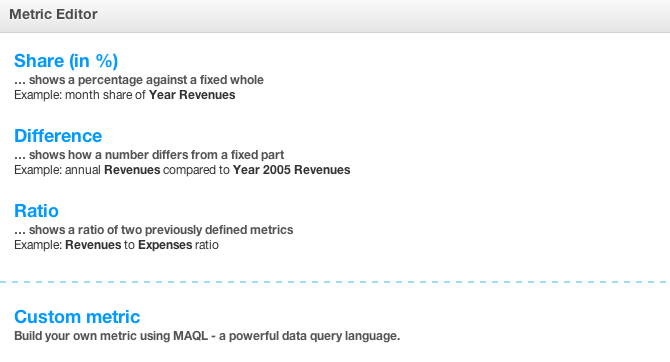
\includegraphics[scale=0.4]{images/metricmenu.png}
\caption{User menu for metric creation}
\label{fig:umm}
\end{figure}

The first 3 options (Share, Difference, Ratio) represent complex metric statements prepared for typical use cases. The fourth option allows you to build your own metric using MAQL DQL.

Each metric is defined by MAQL (MAQL DQL) and consists of 2 main parts -- aggregation and filters (optional).

\subsection{Metrics}
Every report is defined by metrics, which determines WHAT will be computed in the report. Since metrics are numbers, they can be used to calculate Sums, Averages, Minimum Values, Maximum Values and so on.

The metrics are divided into Global Metrics and Report-Specific Metrics whit no difference on the functionality level.

\begin{itemize}
\item \emph{Global Metric} a metric that has been created and is available for all reports,
\item \emph{Report Specific Metric} a metric that has been user-defined for the current report. A Report Specific Metric can be added to the list of global metrics after creation.
\end{itemize}

The only difference is that Global Metrics are available to be used in other reports, while Report Specific Metrics are available only in the current report. Users wanting to use a similar metric will need to create it again in the other report. If you deletes a global metric that is used in a report, the metric is converted to the local metric in the report.

\begin{figure}[htb]
\centering
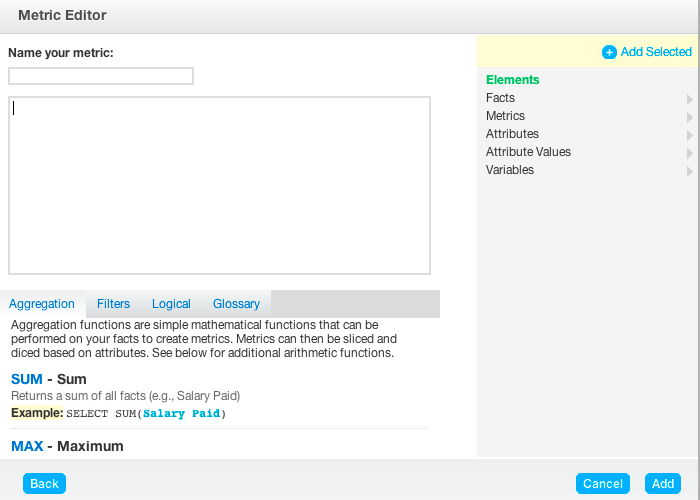
\includegraphics[scale=0.4]{images/metriceditor.png}
\caption{Custom metric editor in GoodData Platform}
\label{fig:medi}
\end{figure}

Following metric definitions examples have semantics used in the custom metric editor in the GoodData platform (as shown on fig.~\ref{fig:medi}). If you like to validate your MAQL DQL statement in the gray pages of your projects, you need to specify the attributes and facts with the brackets as in previous sections of this reference. 

\subsection{Aggregation}
GoodData reports are multi-dimensional pivot tables and each metric must define an aggregation.
\paragraph*{Aggregation} Data aggregation is the process in which information is gathered and expressed in a summary form, or the procedure where data values are grouped with the goal of managing each data unit as a single entity. Sales is a key metric which can be aggregated by Day, Month, Quarter, etc. For aggregation, we do use aggregation function similar to SQL functions but much more intuitive way.\\

You can specify the level at which the data are aggregated. In other words, you can take a~look at the data aggregated by US state, county, city or ZIP levels. You can aggregate by multiple attributes at the same time. For example, you can define your metric to show yearly Payments by Departments. The default aggregation is the whole data set (e.g. one number for the entire country and all years).

\textbf{\emph{syntax}}  \hspace{.9cm}\verb=SELECT FUNCTION(project_fact);=

\textbf{\emph{example}}  \hspace{.55cm}\verb=SELECT AVG(Payment);=

Metrics can then be sliced and diced based on attributes. The following description includes all supported arithmetic functions.

\paragraph*{SUM} Returns a sum of all facts (e.g., Sales)

\textbf{\emph{syntax}}  \hspace{.9cm}\verb=SELECT SUM(project_fact);=

\textbf{\emph{example}}  \hspace{.6cm}\verb=SELECT SUM(Payment);=

\paragraph*{MAX} Returns the maximum value of all facts in the set (e.g., Sales)

\textbf{\emph{syntax}}  \hspace{.9cm}\verb=SELECT MAX(project_fact);=

\textbf{\emph{example}}  \hspace{.6cm}\verb=SELECT MAX(Payment);=

\paragraph*{MIN} Returns the minimum value of all numbers in the set (e.g., Sales)

\textbf{\emph{syntax}}  \hspace{.9cm}\verb=SELECT MIN(project_fact);=

\textbf{\emph{example}}  \hspace{.6cm}\verb=SELECT MIN(Payment);=

\paragraph*{AVG} Returns the average value of all numbers in the set (e.g., Sales)

\textbf{\emph{syntax}}  \hspace{.9cm}\verb=SELECT AVG(project_fact);=

\textbf{\emph{example}}  \hspace{.6cm}\verb=SELECT AVG(Payment);=

\subsubsection{COUNT} 

Globally COUNT returns a count of values for a selected attribute (e.g., as shown on the first syntax definition). But in GoodData, there is an option to pass a second attribute in COUNT definition, referring to the data set where you would like to perform the count (as shown on the second syntax definition).

\textbf{\emph{syntax}}  \hspace{.9cm}\verb=SELECT COUNT(project_attribute);=

\textbf{\emph{example}}  \hspace{.6cm}\verb=SELECT COUNT(Employees);=

This example counts the number of rows entering that are being aggregated (e.g. Employees). In it's default incarnation, it will count the number of unique values in an attribute.

\textbf{\emph{example}}  \hspace{.5cm}\verb=SELECT COUNT(Employees);=

If you use the count function with a primary key of it's dataset (specified as a Connection Point) then this will count the number of rows of that dataset, but now you will receive the number of unique records in that column.

\begin{figure}[htb]
\centering
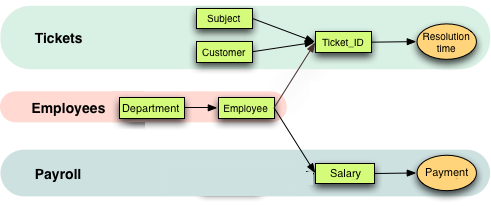
\includegraphics[scale=0.6]{images/hr_extend.png}
\caption{HR demo project LDM -- extended version}
\label{fig:hrldme}
\end{figure}

The issue gets a bit more complicated with multiple datasets. Let's say we have a shared dataset -- for example the Employees dimension. It is connected to both Tickets dataset (support tickets were handled by employees) and to Salary dataset, containing salary data. You can see the extended LDM on figure \ref{fig:hrldme}.

Now with the enhanced LDM, adding a metric \verb=SELECT COUNT(Employee)= to a report will render both dataset Tickets and Salary unusable. The reason is that COUNT will scan all lines of the Employee attribute, but only some of them might be actually connected to \verb=Ticket_ID= or \verb=Salary_ID=. Thus, a second, optional (but very useful) parameter is used in the COUNT function:

\textbf{\emph{syntax}}  \hspace{.9cm}\verb=SELECT COUNT(project_attribute1, project_attribute2);=

\textbf{\emph{example}}  \hspace{.5cm}\verb=SELECT COUNT(Employee,Salary_ID)=

This will count the number of unique employees that are listed in the Salary dataset (connected to \verb=Salary_ID=). As a result, no employees have corresponding rows to the Salary dataset scope are used and you can use all other attributes/metrics from the dataset.

\subsection{Simple Arithmetic}
Once a fact has been aggregated and saved as a metric, it can be used in additional computations. You can modify the result by adding to it, multiplying it, etc. using supported mathematical operators: +, -, *, /.

\textbf{\emph{syntax}}  \hspace{.9cm}\verb=SELECT project_metric1 Operator project_metric2;=

\textbf{\emph{example}} \hspace{.9cm}\verb=SELECT Revenues - Costs;=

\textbf{\emph{example}} \hspace{.9cm}\verb=SELECT Profit * 0.03;= 

\noindent Where Revenues, Costs and Profit are previously defined metrics.

\subsection{Filters}
Filters allow us to narrow the set of data from which the metric is computed. We can also combine filters as itself (see the section \ref{operators}) and use them for conditional filtering. It's also possible to use the time macros (section \ref{timemcr}) along with some simple arithmetic (e.g., using \verb={Previous}= is the same as \verb={This} - 1=). 

\subsubsection{Conditional filtering}
Filtering is about defining the set of data that you are going to analyse. You can specify one or more expressions that apply to the attributes or metrics. 

\textbf{\emph{syntax}}  \hspace{.9cm}\verb=SELECT project_metric WHERE <expression>=

For example you can specify that your metric is going to only compute the Department for HQ Marketing and HQ Human Resources. This limitation is defined in the expression clause. The expression clause can contain attributes, facts, metrics, functions, and logical operators (AND, OR, NOT), operators >, <, >=, <=, =, IN, and NOT IN functions.

Payments for year 2006 and first four months of 2007 are counted by following metric 

\textbf{\emph{example}}  \hspace{.9cm}\verb=SELECT SUM(Payment) WHERE Year= = \verb=2006 =

\hspace{2.2cm}\verb=	OR Month IN (January 2007, February 2007,= 

\hspace{2.2cm}\verb=	March 2007, April 2007);=

You can also combine the dates with facts as in this metric, where we sum all the big payments (higher that 10000) for year 2006 and first four months of 2007.

\textbf{\emph{example}}  \hspace{.9cm}\verb=SELECT SUM(Payment) WHERE Year= = \verb=2006 =

\hspace{2.2cm}\verb=	OR Month IN (January 2007, February 2007,= 

\hspace{2.2cm}\verb=	March 2007, April 2007) AND (Payment > 10000);=

For more examples see the section \ref{operators} at page \pageref{operators}.

We can use these all of the previous clauses to create fixed numbers which can be used in other computations to create complex metrics. Fixing numbers is achieved by locking the aggregation level to an attribute in one or more dimensions. This lock is made with \verb=BY= clause.

\subsection{BY Clause}
By default, each metric is aggregated over a scope of inheritance by it's position in the pivot table. The intersection (resulting set) of \verb=Month(March)= and \verb=Department(HQ Marketing)= will aggregate all rows that have those corresponding attribute values. This allows metrics to be easily drilled into (drill into March to individual days and the metric starts showing numbers for individual days). You might want to override this behaviour though when using the metric as part of some larger calculation.

\verb=BY= in fact locks the value of the metric at the aggregation level specified by the attribute after the \verb=BY= clause. Multiple attributes separated by commas from different dimensions can be specified. Please note that if you lock the value by Year and set the active report to display at a lower aggregation level (e.g., Month), the numbers returned would be the computed value for the whole Year.

\textbf{\emph{syntax}}  \hspace{.9cm}\verb=SELECT project_metric BY project_attribute;=

\textbf{\emph{example}}  \hspace{.9cm}\verb=SELECT Payment BY Year;=

\textbf{\emph{example}}  \hspace{.9cm}\verb=SELECT Payment / (SELECT Payment BY Year);=

The second metric example returns variable Payment (determined by how the metric is sliced and diced in the report) divided by fixed metric \verb=Yearly Payment=. The following example uses the extended version of LDM (see figure~\ref{fig:hrldme} on page~\pageref{fig:hrldme}) example is solving situation when we need to know how many hours were spent on resolving tickets in a particular month, out of all hours in a quarter -- we need both the month and quarter aggregation levels in a metric:

\textbf{\emph{example}}  \hspace{.9cm}\verb=SELECT (SELECT SUM(Resolution time)) /=

\hspace{2.4cm}\verb=(SELECT SUM(Resolution time) BY Quarter);=

This metric results in following table. For better orientation we also added two simple aggregation metrics \verb=SELECT SUM(Resolution time) BY Quarter=\\ and \verb=SELECT SUM(Resolution time)= for the whole resolution time.

\begin{figure}[htb]
\centering
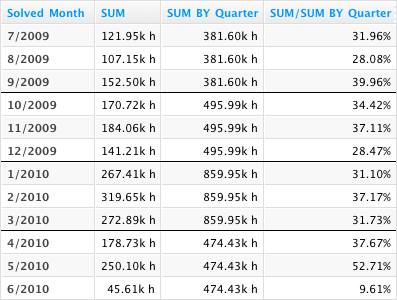
\includegraphics[scale=0.6]{images/by-metric.png}
\caption{Results table of share (\%) metric with BY clause}
\label{fig:share}
\end{figure}

You can see that the \verb=SELECT SUM(Resolution time) BY Quarter= metric displays the identical result for all month in the same quarter, since it's computing results for all months that belong into that quarter. If the report's aggregation level is higher then the one defined in the metric \verb=BY= clause, the metric's aggregation is ignored. 

Continuing with this example, if we replace the Month attribute with a Year attribute, the differences between the metrics will be ignored.  We say that the \verb=BY= clause forces the lowest granularity of the metric to the value for the entire quarter. The situation is shown on following figure. 

\begin{figure}[htb]
\centering
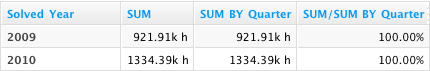
\includegraphics[scale=0.6]{images/by-ignored.png}
\caption{Results table of share (\%) metric with BY Year}
\label{fig:share_ign}
\end{figure}

This metric SUMs all the Payments across whole data set, it means, that it sums Payments from each quarter (e.\,g. Q1, Q2) in all years in the data set.

\textbf{\emph{example}}  \hspace{.9cm}\verb=SELECT SUM(Payment) BY Quarter;=

\noindent The \verb=BY= clause supports multiple attributes. For example the

\textbf{\emph{example}}  \hspace{.9cm}\verb=SELECT SUM(Payment) BY Quarter, Department;=

\noindent forces aggregation to the Quarter and Department levels. If you add this metric to a report with the Department attribute in the rows and the Year attribute in columns, you'll see different numbers for each cell (as on following figure). 

\begin{figure}[htb]
\centering
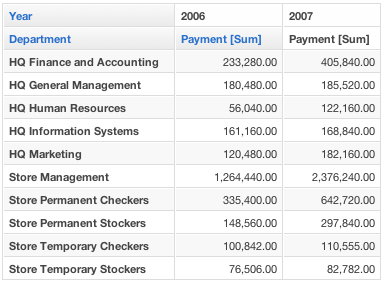
\includegraphics[scale=0.6]{images/qDep.png}
\caption{Sum of all Payments BY Quarter and Department}
\label{fig:qDep}
\end{figure}

Once you change the Year to Month or Day then values for all months or days are going to be the same because of the forced aggregation levels. Once you go below the lock level, the values are going to be the same for these children attributes. Obviously, the report with Month and Department attributes shows all the same numbers.

\begin{figure}[htb]
\centering
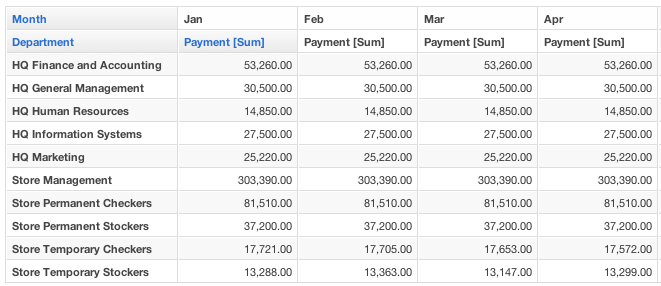
\includegraphics[scale=0.6]{images/qDepM.png}
\caption{Sum of all Payments BY Quarter and Department changed to Month}
\label{fig:qDepM}
\end{figure}

\subsubsection{BY ALL Clause}
In short, the \verb=BY Quarter= clause stops breaking down the payments amounts by anything smaller than a quarter (e.\,g. months and days). \verb=BY ALL= clause locks the value of the metric at the highest possible aggregation level in that hierarchy (one dimension). Let's say we'd like to create showing percentage of Resolution time not just out of the Quarter or Year, but all time. Since the highest-level attribute in the date dimension is Year, we need a new construct \verb=BY ALL=.

There is one problem with this approach. One might need to compute yearly sales as a percentage of total sales. There is a slight problem as "year" is the topmost attribute in the time hierarchy. So we do not have anything above it for our \verb=BY= clause. Fortunately there is a magic \verb=ALL= keyword that helps us handle such situations. 

\verb=ALL= keyword forces aggregation of the whole data set for a particular hierarchy defined after the \verb=BY ALL= clause. So the metric

\textbf{\emph{example}}  \hspace{.9cm}\verb=SELECT SUM(Payment) BY ALL Year;=

\noindent always shows the same value (the total of salary per the whole dataset) no matter what time attribute you put in your report.

However, if you substitute the Department attribute for the Year attribute to the report, the result is the same as in case of simple \verb=SUM(Payment) metric=. No aggregation level is forced, since Department is not part of the time (Year) hierarchy. Obviously, if we were to use the \verb=SUM(Payment) BY ALL Department=, then aggregation by department would be forced and the report would show the same value for all departments.

This fixes the aggregation for all years, but still can break down by attributes from other dimensions. This is best shown by adding a second attribute from a different dimension into our report

\textbf{\emph{example}}  \hspace{.9cm}\verb=SELECT SUM(Payment) BY ALL Year;=\\

\subsubsection{BY project\_attribute ALL IN ALL OTHER DIMENSIONS}
This complements the \verb=BY= statement by specifying how the aggregation of the metrics should be calculated in all other dimensions not previously specified in the \verb=BY= statement. Omitting \verb=ALL IN ALL OTHER DIMENSIONS= allows the metric to be sliced and diced in other dimensions.

\textbf{\emph{syntax}}  \hspace{.9cm}\verb=SELECT project_metric=

\hspace{2.2cm}\verb=BY project_attribute ALL IN ALL OTHER DIMENSIONS;=

It is useful when we need to create a metric that is fixed at highest aggregation (undrillable) in all dimension but the date dimension, where it is fixed at the Quarter level:

\textbf{\emph{example}}  \hspace{.9cm}\verb=SELECT SUM(Resolution time)=

\hspace{2.4cm}\verb=BY Quarter, ALL IN ALL OTHER DIMENSIONS;=

Another similar construct is \verb=BY ALL IN ALL OTHER DIMENSIONS EXCEPT=\\ \verb=FOR project_attribute=. The only difference between these two constructs is that\\ \verb=EXCEPT FOR project_attribute= preserves natural aggregation in the dimension specified by the \verb=project_attribute= (e.\,g., date dimension specified by Quarter) but \verb=Quarter,= \verb=ALL IN ALL OTHER DIMENSIONS= construct will never drill in the date dimension bellow the level specified by Quarter.

\textbf{\emph{syntax}}  \hspace{.9cm}\verb=SELECT project_metric=

\hspace{2.2cm}\verb=BY ALL IN ALL OTHER DIMENSIONS=

\hspace{2.2cm}\verb=EXCEPT [FOR] project_attribute=

By adding the \verb=EXCEPT FOR project_attribute= to the \verb=BY ALL= clause specifies an exception where the metric will be sliced and diced by the specified attribute (and its hierarchy) if the attribute is contained in the report (or any other attribute from the same hierarchy).

\textbf{\emph{example}}  \hspace{.9cm}\verb=SELECT Payment=

\hspace{2.2cm}\verb=	BY ALL IN ALL OTHER DIMENSIONS=

\hspace{2.2cm}\verb=	EXCEPT FOR Date;=

\subsubsection{BY ALL IN ALL OTHER DIMENSIONS}
This clause locks the value of the metric at the highest possible aggregation level across all dimensions. Therefore, this returns a grand total that is indivisible. Simply said, BY ALL IN ALL OTHER DIMENSIONS clause excludes attributes one by one can be pretty annoying in projects with hundreds of attributes.

\textbf{\emph{syntax}}  \hspace{.9cm}\verb=SELECT project_metric BY ALL IN ALL OTHER DIMENSIONS=

\textbf{\emph{example}}  \hspace{.9cm}\verb=SELECT Payment /=

\hspace{2.4cm}\verb=(SELECT Payment BY ALL IN ALL OTHER DIMENSIONS);=

In this example, this metric returns variable Revenues (determined by how the metric is sliced and diced in the report) divided by a fixed grand total for Revenues.

If you want to exclude all attributes, you can use the OTHER and IN ALL OTHER DIMENSIONS keywords and define metric that forces aggregation level to the whole data set in all dimensions: 

\textbf{\emph{example}}  \hspace{.9cm}\verb=SELECT SUM(Sale Amount) BY ALL IN ALL OTHER DIMENSIONS;=

\noindent Metric that forces aggregation level to Month in the time dimension and to the whole data set in all other dimensions: 

\textbf{\emph{example}}  \hspace{.9cm}\verb=SELECT SUM(Sale Amount) BY Month,=

\hspace{2.2cm}\verb=	ALL IN ALL OTHER DIMENSIONS;=

\noindent Metric that computes a percentage to the whole data set for any attribute that you add to the report: 

\textbf{\emph{example}}  \hspace{.9cm}\verb=SELECT  SUM(Sale Amount) /=

\hspace{2.2cm}\verb=	(SELECT SUM(Sale Amount)=

\hspace{2.2cm}\verb=	BY ALL IN ALL OTHER DIMENSIONS);=

\subsubsection{WITHOUT PARENT FILTER}
Simply said WITHOUT PARENT FILTER clause excludes filters of active report. This clause allows to compute the metric with no regard to any filter or metric currently in place in the active report. It's really handy when we are reusing any metric in the report and we need to omit any applied filters. 

\textbf{\emph{syntax}}  \hspace{.9cm}\verb=SELECT project_metric BY ALL project_attribute=

\hspace{2.2cm}\verb=WITHOUT PARENT FILTER;=

This clause results the amount (e.g. SUM) for all Years even if some Years were filtered out of the active report.

\textbf{\emph{example}}  \hspace{.9cm}\verb=SELECT Payment -=

\hspace{2.4cm}\verb=(SELECT Payment BY ALL Year=

\hspace{2.4cm}\verb=WITHOUT PARENT FILTER);=

\end{document}
